\documentclass[tikz,border=12pt]{standalone}
\usepackage[T1]{fontenc}
\usepackage{mathpazo}
\usepackage{amsmath,amssymb}
\usetikzlibrary{arrows.meta, positioning, calc}

\definecolor{stblue}{HTML}{7B97AD}
\definecolor{rwgold}{HTML}{B8995E}
\definecolor{sage}{HTML}{7A9A7E}
\definecolor{dkbrown}{HTML}{3D3530}
\definecolor{wmgray}{HTML}{7B7067}
\definecolor{cream}{HTML}{F9F6F0}
\definecolor{border}{HTML}{D4C9B8}

\begin{document}
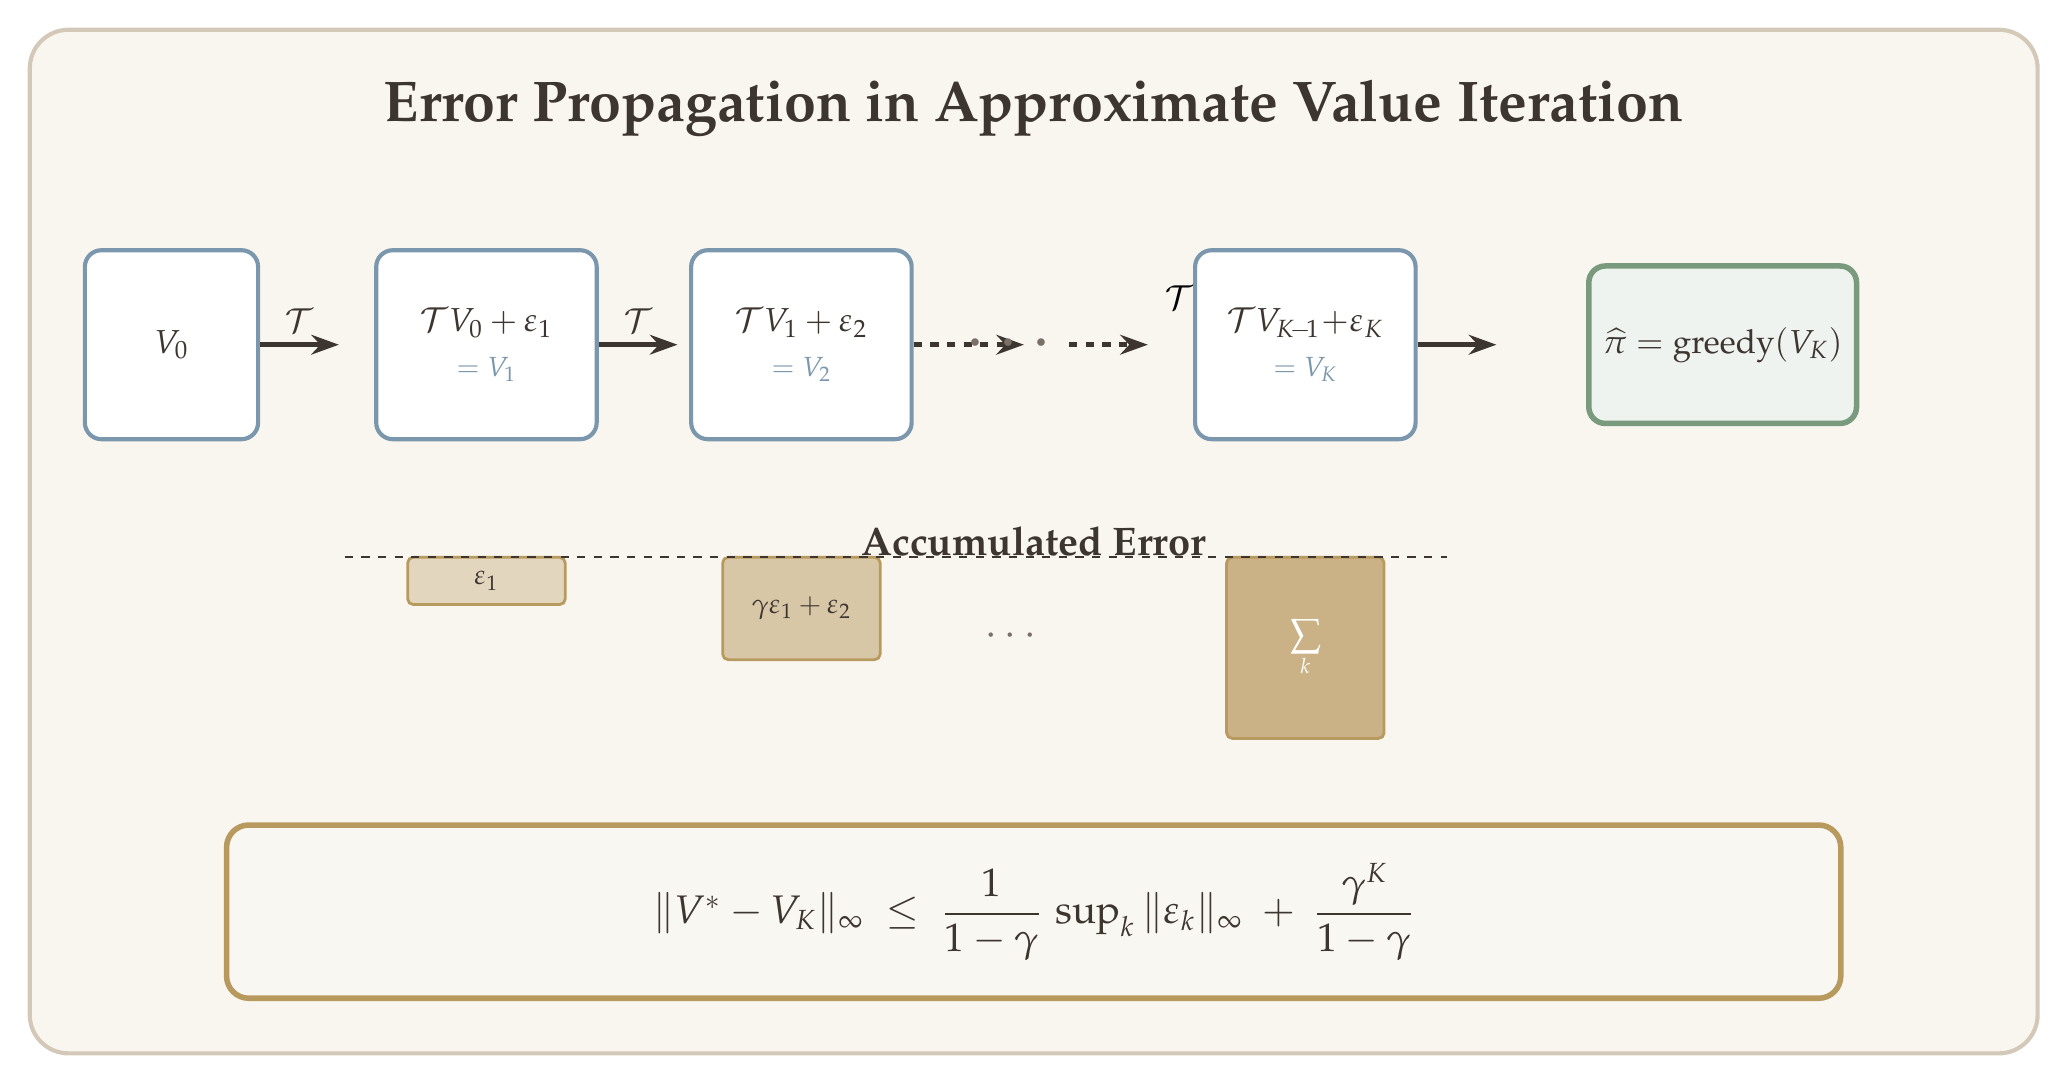
\begin{tikzpicture}[
  >={Stealth[length=3.5mm, width=2.5mm]},
  iterbox/.style={draw=stblue, line width=1.5pt, fill=white, rounded corners=6pt,
    minimum width=28mm, minimum height=24mm, align=center, inner sep=4pt,
    font=\large, text=dkbrown},
  arr/.style={->, line width=1.8pt, dkbrown},
]

% Background
\fill[cream, rounded corners=14pt] (-1.0,-7.5) rectangle (24.5,5.5);
\draw[border, rounded corners=14pt, line width=1.5pt] (-1.0,-7.5) rectangle (24.5,5.5);

% Title
\node[font=\huge\bfseries, text=dkbrown] at (11.75,4.5)
  {Error Propagation in Approximate Value Iteration};

% =============================================
% Pipeline: V_0 -> TV_0 + e_1 = V_1 -> ... -> V_K -> greedy
% =============================================

% V_0
\node[iterbox, minimum width=22mm] (v0) at (0.8,1.5)
  {$V_0$};

% Arrow T
\draw[arr] (v0.east) -- ++(1.0,0) node[midway, above, font=\large] {$\mathcal{T}$};

% V_1 = TV_0 + e_1
\node[iterbox] (v1) at (4.8,1.5)
  {$\mathcal{T}V_0 + \varepsilon_1$\\[2pt]
   {\normalsize\color{stblue} $= V_1$}};

% Arrow T
\draw[arr] (v1.east) -- ++(1.0,0) node[midway, above, font=\large] {$\mathcal{T}$};

% V_2
\node[iterbox] (v2) at (8.8,1.5)
  {$\mathcal{T}V_1 + \varepsilon_2$\\[2pt]
   {\normalsize\color{stblue} $= V_2$}};

% Dots
\draw[arr, dashed] (v2.east) -- ++(1.4,0);
\node[font=\Huge, text=wmgray] at (11.5,1.5) {$\cdots$};
\draw[arr, dashed] (12.2,1.5) -- ++(1.0,0);

% Arrow T
\node at (13.6,2.1) [font=\large] {$\mathcal{T}$};

% V_K
\node[iterbox] (vk) at (15.2,1.5)
  {$\mathcal{T}V_{K\!-\!1}\! +\! \varepsilon_K$\\[2pt]
   {\normalsize\color{stblue} $= V_K$}};

% Arrow to greedy
\draw[arr] (vk.east) -- ++(1.0,0);

% Greedy policy
\node[draw=sage, line width=2pt, fill=sage!12, rounded corners=6pt,
  minimum width=34mm, minimum height=20mm, align=center, inner sep=5pt,
  font=\large, text=dkbrown] (greedy) at (20.5,1.5)
  {\textbf{$\widehat{\pi} = \operatorname{greedy}(V_K)$}};

% =============================================
% Error accumulation bars
% =============================================
\node[font=\Large\bfseries, text=dkbrown] at (11.75,-1.0)
  {Accumulated Error};

% Bar 1
\fill[rwgold!40, rounded corners=2pt] (3.8,-1.8) rectangle (5.8,-1.2);
\draw[rwgold, line width=1pt, rounded corners=2pt] (3.8,-1.8) rectangle (5.8,-1.2);
\node[font=\normalsize, text=dkbrown] at (4.8,-1.5) {$\varepsilon_1$};

% Bar 2
\fill[rwgold!55, rounded corners=2pt] (7.8,-2.5) rectangle (9.8,-1.2);
\draw[rwgold, line width=1pt, rounded corners=2pt] (7.8,-2.5) rectangle (9.8,-1.2);
\node[font=\normalsize, text=dkbrown] at (8.8,-1.85) {$\gamma\varepsilon_1 + \varepsilon_2$};

% Bar K (sum)
\fill[rwgold!75, rounded corners=2pt] (14.2,-3.5) rectangle (16.2,-1.2);
\draw[rwgold, line width=1pt, rounded corners=2pt] (14.2,-3.5) rectangle (16.2,-1.2);
\node[font=\normalsize, text=white] at (15.2,-2.35) {$\displaystyle\sum_{k}$};

% Baseline
\draw[dkbrown, line width=0.8pt, dashed] (3.0,-1.2) -- (17.0,-1.2);

% Dots between bars
\node[font=\Large, text=wmgray] at (11.5,-2.2) {$\cdots$};

% =============================================
% Bottom: Error bound formula
% =============================================
\draw[rwgold, line width=2pt, rounded corners=8pt, fill=rwgold!8]
  (1.5,-6.8) rectangle (22.0,-4.6);

\node[font=\Large, text=dkbrown, align=center] at (11.75,-5.7)
  {$\|V^* - V_K\|_\infty \;\leq\; \dfrac{1}{1-\gamma}\,\sup_k \|\varepsilon_k\|_\infty \;+\; \dfrac{\gamma^K}{1-\gamma}$};

\end{tikzpicture}
\end{document}
